% LaTeX Template For MATH 490 @ VCU
\documentclass[11pt]{article}

\usepackage{hyperref}
\usepackage{amsmath}
\usepackage{amsthm}
\usepackage{amssymb}
\usepackage{enumerate}
\usepackage{enumitem}
\usepackage{titlesec}
\usepackage{multicol}
\usepackage{multirow}
\usepackage{mathtools}
\usepackage{mdframed}
\usepackage{tocloft}
\usepackage{tcolorbox}
\usepackage{extarrows}

\setlist{nosep}
\setlist[enumerate]{label=\alph*.}

\renewcommand{\arraystretch}{0.75}

\definecolor{defcolor}{RGB}{255,236,236}    % light red
\definecolor{ngtcolor}{RGB}{255,242,242}    % lighter red
\definecolor{lnkcolor}{RGB}{0,0,180}        % blue
\definecolor{thmcolor}{RGB}{236,236,255}    % light blue
\definecolor{lemcolor}{RGB}{239,239,255}    % lighter blue
\definecolor{procolor}{RGB}{242,242,255}    % lighter lighter blue
\definecolor{crlcolor}{RGB}{245,245,255}    % lighter lighter lighter blue
\definecolor{xmpcolor}{RGB}{255,240,225}    % light orange
\definecolor{rmkcolor}{RGB}{233,255,235}    % light green
\definecolor{axicolor}{RGB}{255,255,233}    % light yellow
\definecolor{notcolor}{RGB}{255,255,244}    % lighter yellow
\definecolor{whacolor}{RGB}{250,250,250}    % lighter gray
\definecolor{reccolor}{RGB}{255,244,255}    % lighter purple

\hypersetup{
    colorlinks,
    citecolor=lnkcolor,
    filecolor=lnkcolor,
    linkcolor=lnkcolor,
    urlcolor=lnkcolor
}

\newtheoremstyle{break}
    {\topsep/1.5} % space above
    {\topsep/2.2} % space below
    {}          % body font
    {}          % indent amount
    {\rmfamily} % theorem head font
    {.}          % punctuation after theorem head
    {0.5em}  % space after theorem head
    {\textbf{\thmname{#1}\thmnumber{ #2}}\thmnote{\text{ (#3)}}}
                % theorem hed spec. (empty = "normal")

\theoremstyle{break}
\newmdtheoremenv{theorem}{Theorem}
\newmdtheoremenv{corollary}[theorem]{Corollary}
\newmdtheoremenv{lemma}[theorem]{Lemma}
\newmdtheoremenv{axiom}[theorem]{Axiom}
\newmdtheoremenv{notation}[theorem]{Notation}
\newmdtheoremenv{definition}[theorem]{Definition}
\newmdtheoremenv{remark}[theorem]{Remark}
\newmdtheoremenv{example}[theorem]{Example}
\newmdtheoremenv{problem}[theorem]{Problem}
\newmdtheoremenv{question}[theorem]{Question}

\DeclareMathOperator{\arcsec}{arcsec}
\DeclareMathOperator{\arccot}{arccot}
\DeclareMathOperator{\arccsc}{arccsc}
\DeclareMathOperator{\interior}{int}
\DeclareMathOperator{\closure}{cl}
\DeclareMathOperator{\boundary}{bd}

\newcommand{\dd}{\text{d}}
\newcommand{\ddi}{\text{$\,$d}}
\newcommand{\qqed}{{\hfill$\blacksquare$}}
\newcommand{\defeq}{\overset{\text{def}}{=}}
\newcommand{\transpose}{\text{T}}

\linespread{1.9}
\setlength{\textwidth}{6.9in}
\setlength{\textheight}{9.2in}
\setlength{\oddsidemargin}{-0.2in}
\setlength{\evensidemargin}{-0.2in}
\setlength{\topmargin}{-0.2in}
\setlength{\headheight}{0in}
\setlength{\headsep}{0in}
\setlength{\footskip}{0.5in}
\setlength{\multicolsep}{6.2pt}
\setlength{\belowdisplayskip}{0pt}
%\setlength{\belowdisplayshortskip}{0pt}
\setlength{\abovedisplayskip}{0pt}
%\setlength{\abovedisplayshortskip}{0pt}

\setcounter{section}{0}
\numberwithin{equation}{theorem}

\makeatletter
\newcommand{\vast}{\bBigg@{4}}
\newcommand{\Vast}{\bBigg@{5}}
\makeatother
\title{Homework 2 of Computational Mathematics}
\author{Chang, Yung-Hsuan\\111652004\\Department of Applied Mathematics}

\begin{document}
\maketitle
\thispagestyle{empty}
\newpage
\pagenumbering{arabic}

\begin{problem}\label{problem 1}
    Use a fixed-point iteration method to determine a solution accurate to within $10^{-2}$ for $x^3-x-1=0$ on $[1, 2]$. Use $p_0=1$.
\end{problem}
\textbf{Solution}. By Algebra, we have
\begin{align*}
    x^3-x-1&=0\\
    x^2&=1+\dfrac{1}{x}\\
    x&=\sqrt{1+\dfrac{1}{x}}
\end{align*}
for $x>0$. We want to find the solution to $f(x)=x$ with $f(x)=\sqrt{1+\dfrac{1}{x}}$. Then, by calculator,
\begin{align*}
    p_1&=\sqrt{2}=1.414,\\
    p_2&=1.307,\\
    p_3&=1.329,\\
    p_4&=1.324,
\end{align*}
which is accurate to within $10^{-2}$ for $x^3-x-1=0$ on $[1, 2]$. \qed


\newpage
\begin{problem}\label{problem 2}
    Use Theorem 2.1 to find a bound for the number of iterations needed to achieve an approximation with accuracy $10^{-3}$ to the solution of $x^3+x-4=0$ lying in the interval $[1, 4]$. Find an approximation to the root with this degree of accuracy.
\end{problem}
\textbf{Solution}. Let $f(x)=x^3+x-4$. Since $f\in C[1, 4]$ and $f(1)\cdot f(4)=(-2)\cdot 64<0$. The Bisection method generates a sequence $\{p_n\}_{n=1}^\infty$ approaches to a zero $p$ of $f$ with
\begin{equation*}
    |p_n-p|\leq\dfrac{4-1}{2^n},\quad\text{when $n\geq 1$}.
\end{equation*}
Then,
\begin{equation*}
    \dfrac{3}{2^n}\leq10^{-3}\implies n\geq\log_2(3000)>11.
\end{equation*}

\begin{center}
    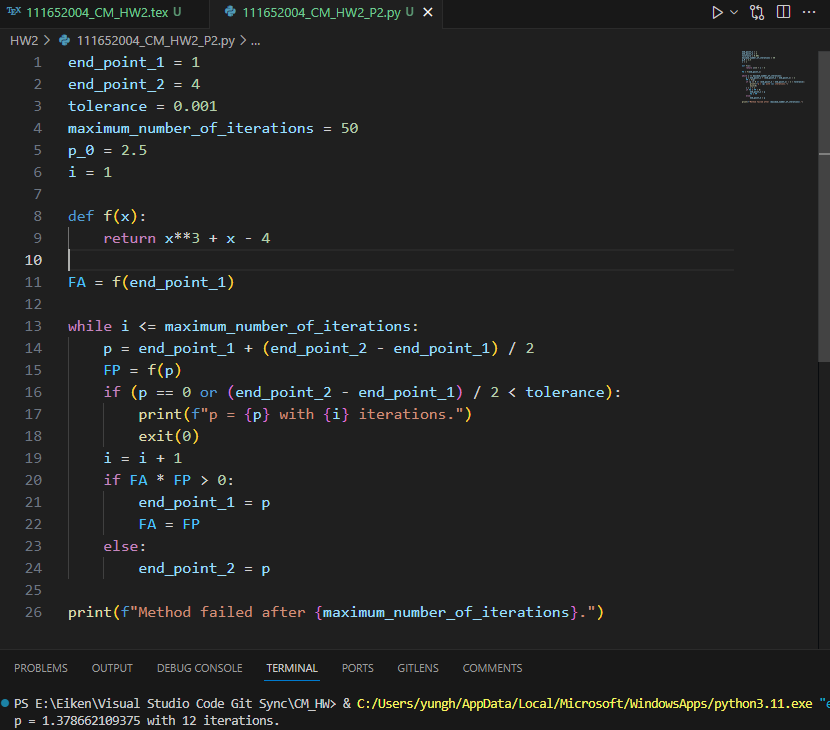
\includegraphics[width=0.9\textwidth]{problem_2_py.png}
\end{center}
Using the bisection method, by Python, $p=1.37866$. \qed


\newpage
\begin{problem}\label{problem 3}
    The following four methods are preposed to compute $21^{1/3}$. Rank them in order, based on their apparent speed of convergence, assuming $p_0=1$.
    \begin{enumerate}
        \item $p_n = \dfrac{20p_{n-1} + \frac{21}{{p_{n-1}}^2}}{21}$
        \item $p_n = p_{n-1} - \dfrac{{p_{n-1}}^3-21}{3{p_{n-1}}^2}$
        \item $p_n = p_{n-1} - \dfrac{{p_{n-1}}^4 - 21p_{n-1}}{{p_{n-1}}^2-21}$
        \item $p_n=\sqrt{\dfrac{21}{p_{n-1}}}$
    \end{enumerate}
\end{problem}
\textbf{Solution}. For a, choose $g_1(x)=\dfrac{20x+\frac{21}{x^2}}{21}=\dfrac{20x}{21}+\dfrac{1}{x^2}$. Then ${g_1}'(x)=\dfrac{20}{21}-\dfrac{2}{x^3}$. Hence $${g_1}'(\sqrt[3]{21})=\dfrac{20}{21}-\dfrac{2}{21}\approx0.86.$$ For b, choose $g_2(x)=x-\dfrac{x^3-21}{3x^2}=\dfrac{2x}{3}+\dfrac{7}{x^2}$. Then ${g_2}'(x)=\dfrac{2}{3}-\dfrac{14}{x^3}$. Hence
$${g_2}'(\sqrt[3]{21})=\dfrac{2}{3}-\dfrac{1}{3}\approx0.33.$$
For c, choose ${g_3}(x)=x-\dfrac{x^4-21x}{x^2-21}=\dfrac{x^3-x^4}{x^2-21}$. Then ${g_3}'(x)=\dfrac{-2x^5+x^4+84x^3-63x^2}{x^4-42x^2+441}$. Hence $${g_3}'(\sqrt[3]{21})\approx5.7.$$ For d, choose ${g_4}(x)=\sqrt{\dfrac{21}{x}}$. Then ${g_4}'(x)=\dfrac{-\sqrt{21}}{2x^{\frac{3}{2}}}$. Hence $${g_4}'(\sqrt[3]{21})=\dfrac{1}{2}.$$ To sum up, the apparent speed of convergence in order is b, d, a, and c does not converge (the derivative at $\sqrt[3]{21}$ is greater than $1$.) \qed


\newpage
\begin{problem}\label{problem 4}
    Use Theorem 2.3 to show that $g(x)=2^{-x}$ has a unique fixed point on $\left[\dfrac{1}{3}, 1\right]$. Use fixed-point iteration to find an approximation to the fixed point accurate to within $10^{-4}$. Use corollary 2.5 to estimate the number of iterations required to achieve $10^{-4}$ accuracy, and compare this theoratical estimate the the number actually needed.
\end{problem}
\textbf{Solution}. We know that $g\in C\left[\dfrac{1}{3}, 1\right]$ and $g(x)\in[0.5, 0.9637]\subseteq\left[\dfrac{1}{3}, 1\right]$ for all $x\in\left[\dfrac{1}{3}, 1\right]$. Then $g$ has at least a fixed point in $[a, b]$. Moreover, $g'(x)$ exists on $\left(\dfrac{1}{3}, 1\right)$. Choose $k=0.7$. Then
\begin{align*}
    \left|\dfrac{\dd}{\dd x}2^{-x}\right|&=\ln2\cdot 2^{-x}\\
    &<\ln2\cdot 2^{-0}\\
    &=\ln2\\
    &<k
\end{align*}
for all $x\in(0, \infty)$. Hence, $g'(x)$ exists on $\left(\dfrac{1}{3}, 1\right)$ and a positive $0<k<1$ exsits with $\left|g'(x)\right|\leq k$ for all $x\in\left(\dfrac{1}{3}, 1\right)$. Then there exists exactly one fixed point in $\left[\dfrac{1}{3}, 1\right]$. It is known the assumption of Theorem 2.4 holds, i.e., $g'(x)$ exists on $\left(\dfrac{1}{3}, 1\right)$ and a positive $0<k<1$ exsits with $\left|g'(x)\right|\leq k$ for all $x\in\left(\dfrac{1}{3}, 1\right)$. By Corollary 2.5, 
\begin{equation*}
    |p_n-p|\leq 0.7^n\max\{0.6-\dfrac{1}{3}, 1-0.6\}.
\end{equation*}
Then,
\begin{equation*}
    0.7^n\max\{0.6-\dfrac{1}{3}, 1-0.6\}\leq 10^{-4} \implies n>23.
\end{equation*}

\begin{center}
    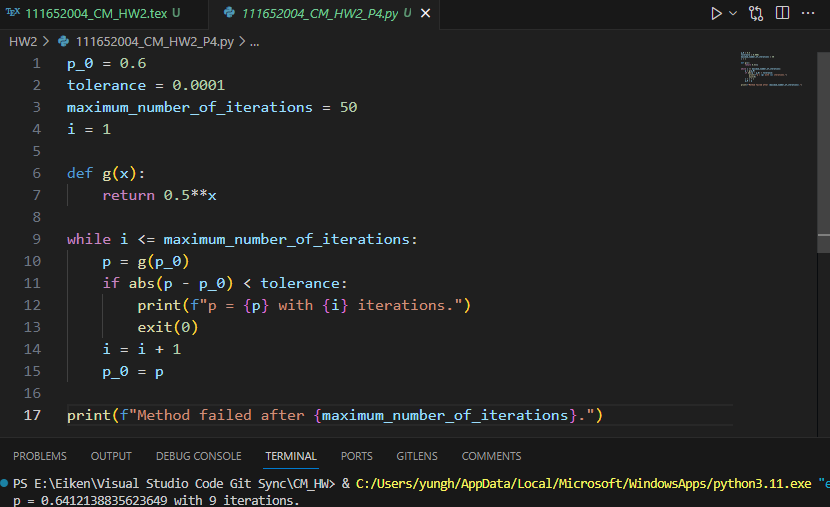
\includegraphics[width=0.9\textwidth]{problem_4_py.png}
\end{center}
By Python, the number of iteration actually needed is 9, which is smaller due to my overestimation for error. \qed


\newpage
\begin{problem}\label{problem 5}
    Let $A$ be a given positive constant and $g(x)=2x-Ax^2$.
    \begin{enumerate}
        \item Show that if fixed-point iteration converges to a nonzero limit, then the limit is $p=\dfrac{1}{A}$, so the inverse of a number can be found using only multiplications and subtractions.
        \item Find an interval about $\dfrac{1}{A}$ for which fixed-point iteration converges, provided $p_0$ is in that interval.
    \end{enumerate}
\end{problem}
\textbf{Solution}.
\begin{enumerate}
    \item Suppose that fixed-point iteration converges to a nonzero limit, say $p$. We want to show that $p=\dfrac{1}{A}$. For the sake of contradiction, suppose $p\ne\dfrac{1}{A}$. Then, by the definition of convergence, we have 
    \begin{equation*}
        p=2p-Ap^2.
    \end{equation*}
    By the fact that $p$ is nonzero, we further have
    \begin{equation*}
        1=2-Ap,
    \end{equation*}
    which implies $Ap=1$, a contradiction.
    \item We have $g(x)=2x-Ax^2$ with $g\in C\left[\dfrac{2}{3A}, \dfrac{4}{3A}\right]$ and then
    \begin{align*}
        g(x)&=-A\left(x+\dfrac{1}{A}\right)^2+\dfrac{1}{A}\\
        &\leq-A\cdot\left(\dfrac{1}{3A}\right)^2+\dfrac{1}{A}\\
        &=\dfrac{1}{A}-\dfrac{1}{9A}\\
        &=\dfrac{8}{9A}.
    \end{align*}
    Hence $g(x)\in\left[\dfrac{2}{3A}, \dfrac{4}{3A}\right]$ for all $x\in\left[\dfrac{2}{3A}, \dfrac{4}{3A}\right]$. In addition, $g'(x)=2-2Ax$ exists on $\left(\dfrac{2}{3A}, \dfrac{4}{3A}\right)$. Then $|g'(x)|<\dfrac{2}{3}$ for all $x\in\left(\dfrac{2}{3A}, \dfrac{4}{3A}\right)$. By the fix-point theorem, the sequence defined by
    $$p_n=g(g_{n-1}),\quad n\geq 1$$ converges to the unique fixed point $\dfrac{1}{A}$ in $\left[\dfrac{2}{3A}, \dfrac{4}{3A}\right]$. \qed
\end{enumerate}


\newpage
\begin{problem}\label{problem 6}
    Show that if $A$ is any positive number, then the sequence defined by
    \begin{equation*}
        x_n=\dfrac{1}{2}x_{n-1}+\dfrac{A}{2x_{n-1}},\quad\text{for $n\geq 1$},
    \end{equation*}
    converges to $\sqrt{A}$ whenever $x_0>0$.
\end{problem}
\textbf{Solution}. Let $A>0$. Let $x_0>0$. Let $k\in\mathbb{N}$. Suppose $x_k>0$. Then $x_{k+1}=\dfrac{1}{2}x_k+\dfrac{A}{2x_k}>0$. Thus $x_k>0$ for all $k\in\mathbb{N}$. By the AM-GM inequality, we have
\begin{equation}
    x_n=\dfrac{1}{2}x_{n-1}+\dfrac{A}{2x_{n-1}}\geq\sqrt{A}
\end{equation}
for all $n\in\mathbb{N}$, and the equation does not hold provided that $x_{n-1}=\sqrt{A}$. We now separate three cases for the initial $x_0$. First, suppose that $x_0=\sqrt{A}$. Then it is obvious that $x_k=\sqrt{A}$ for all $k\in\mathbb{N}$. Hence $x_k\to\sqrt{A}$ as $k\to\infty$. We now deal with $x_0\ne\sqrt{A}$. Suppose $x_0\ne\sqrt{A}$. Then by (6.1), $x_k>\sqrt{A}$ for all $k\in\mathbb{N}$. Thus
\begin{align*}
    x_{k+1}-x_{k}&=\dfrac{1}{2}x_{k}+\dfrac{A}{2x_{k}}-x_{k}\\
    &=\dfrac{A}{2x_{k}}-\dfrac{1}{2}x_{k}\\
    &=\dfrac{1}{2x_{k}}\left(A-{x_{k}}^2\right)\\
    &<0
\end{align*}
for all $k\in\mathbb{N}$, which implies that $\{x_n\}$ is decreasing. Since $\{x_n\}$ is bounded and monotone, by the monotone convergence theorem, $\{x_n\}$ converges. Say the limit is $L$. Then by the recursive relation, $L=\dfrac{1}{2}L+\dfrac{A}{2L}$, which implies $L=\pm\sqrt{A}$. Since $\{x_n\}\subseteq[\sqrt{A}, \infty)$, the limit is $\sqrt{A}$. \qed

\newpage
\begin{problem}\label{problem 7}
    Let $f(x)=-x^3-\cos x$. With $p_0=-1$ and $p_1=0$, find $p_3$.
    \begin{enumerate}
        \item Use the Secant method.
        \item Use the method of False Position.
    \end{enumerate}
\end{problem}
\textbf{Solution}.
\begin{enumerate}
    \item By the algorithm of the secant method, we have the formula
    \begin{equation*}
        p_n=p_{n-1}-f(p_{n-1})\cdot\dfrac{p_{n-1}-p_{n-2}}{f(p_{n-1})-f(p_{n-2})}.
    \end{equation*}
    Thus, by calculator,
    \begin{align*}
        p_2&=0-f(0)\cdot\dfrac{0-(-1)}{f(0)-f(-1)}\\
        &=\dfrac{1}{-1-(1-\cos(-1))}\\
        &=\dfrac{1}{-2+\cos(-1)}\\
        &\approx-0.685,
    \end{align*}
    and
    \begin{align*}
        p_3&=-0.685-f(-0.685)\cdot\dfrac{-0.685-0}{f(-0.685)-f(0)}\\
        &\approx-1.252.
    \end{align*}
    \item We first check that $f(-1)$ and $f(0)$ has different sign. By calculator,
    \begin{equation*}
        f(-1)\approx0.45
    \end{equation*}
    and
    \begin{equation*}
        f(0)=-1.
    \end{equation*}
    By the algorithm of the false position, we have the formula
    \begin{equation*}
        p_n=p_{n-1}-f(p_{n-1})\cdot\dfrac{p_{n-1}-p_{n-2}}{f(p_{n-1})-f(p_{n-2})}.
    \end{equation*}
    Thus, by calculator,
    \begin{align*}
        p_2&=0-f(0)\cdot\dfrac{0-(-1)}{f(0)-f(-1)}\\
        &=\dfrac{1}{-1-(1-\cos(-1))}\\
        &=\dfrac{1}{-2+\cos(-1)}\\
        &\approx-0.685.
    \end{align*}
    By calculator, $f(p_2)\approx-0.453$. Hence the endpoints become $-0.685$ and $0$. By calculator,
    \begin{align*}
        p_3&=0-f(0)\cdot\dfrac{0-(-0.685)}{f(0)-f(-0.685)}\\
        &\approx-0.841.
    \end{align*}
    \qed
\end{enumerate}


\newpage
\begin{problem}\label{problem 8}
    Problems involving the amount of money required to pay off a mortgage over a fixed period of time involve the formula
    \begin{equation*}
        A=\dfrac{P}{i}\left(1-(1+i)^{-n}\right),
    \end{equation*}
    known as an \emph{ordinary annuity equation}. In this equation, $A$ is the amount of the mortgage, $P$ is the amount of each payment, and $i$ is the interest rate per period for the $n$ payment periods. Suppose that a 30-year home mortgage in the amount of \$135,000 is needed and that the borrower can afford house payments of at most \$1000 per month. What is the maximal interest rate the borrower can afford to pay?
\end{problem}
\textbf{Solution}. Using the information, we have 
\begin{equation*}
    A=135000, \qquad P=1000, \qquad \text{and}\quad n=360,
\end{equation*}
and we aim to solve for $i$ in the following equation
\begin{equation}
    f(i)=0
\end{equation}
with $f(i)=135000i-1000\left(1-(1+i)^{-360}\right)$. We use the bisection method with Python to solve (8.1). By calculator, we have 
\begin{equation*}
    f(0.001)\approx-167.2
\end{equation*}
and
\begin{equation*}
    f(0.01)\approx377.8.
\end{equation*}
Since $f$ is continuous, by the intermediate value theroem, there is a solution to $f(i)=0$ in $(0.001, 0.01)$. By Python, we have that the solution (month interest) to (8.1) is approximately $0.675\%$.
\begin{center}
    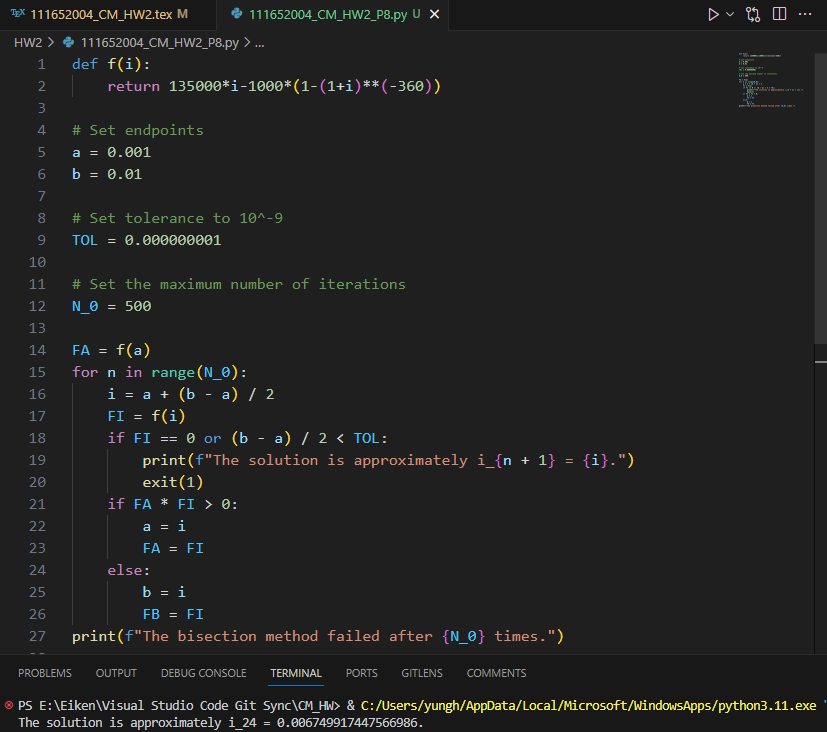
\includegraphics[width=0.9\textwidth]{problem_8_py.png}
\end{center}
\qed



\newpage
\begin{problem}\label{problem 9}$\ $
    \begin{enumerate}
        \item Show that for any positive integer $k$, the sequence defined by $p_n=\dfrac{1}{n^k}$ converges linearly to $p=0$.
        \item Show that the sequence $p_n=10^{-2^n}$ converges quadratically to $0$.
    \end{enumerate}
\end{problem}
\textbf{Solution}.
\begin{enumerate}
    \item Let $k\in\mathbb{N}$. It is clear that $\dfrac{1}{n^k}\to0$ as $n\to\infty$. Choose $\alpha=1$. Then
    \begin{align*}
        \lim_{n\to\infty}\dfrac{\left\lvert\frac{1}{(n+1)^k}-0\right\rvert}{\left\lvert\frac{1}{n^k}-0\right\rvert^1}&=\left(\lim_{n\to\infty}\dfrac{n}{n+1}\right)^k\\
        &=1.
    \end{align*}
    Hence the sequence is lienarly convergent.
    \item It is clear that $10^{-2^n}\to0$ as $n\to\infty$. Choose $\alpha=2$. Then
    \begin{align*}
        \lim_{n\to\infty}\dfrac{\left\lvert10^{-2^{n+1}}-0\right\rvert}{\left\lvert10^{-2^n}-0\right\rvert^2}&=\lim_{n\to\infty}10^{-2^{n+1}+2^{n+1}}\\
        &=1.
    \end{align*}
    Since the asymptotic error constant is $\lambda=1$, the sequence is quadratically convergent. \qed
\end{enumerate}


\newpage
\begin{problem}\label{problem 10}$\ $
    \begin{enumerate}
        \item The following sequences are linearly convergent. Generate the first five terms of the sequence $\{\hat{p_n}\}$ using Aitken's $\Delta^2$ method.
        \begin{equation*}
            p_0=0.5, \quad p_n=\cos(p_{n-1}), \quad n\geq 1
        \end{equation*}
        \item Use Steffensen's method to find, to an accuracy of $10^{-4}$, the root of $x^3-x-1=0$ that lies in $[1, 2]$.
    \end{enumerate}
\end{problem}
\textbf{Solution}.
\begin{enumerate}
    \item Aitken's $\Delta^2$ method requires the first $7$ terms of $\{p_n\}$. By calculator, we have the table:
    \begin{center}
        \begin{tabular}{|c|c|}
            \hline
            $n$ & $p_n$ \\
            \hline
            $0$ & $0.5$ \\
            \hline
            $1$ & $0.877583$ \\
            \hline
            $2$ & $0.639012$ \\
            \hline
            $3$ & $0.802685$ \\
            \hline
            $4$ & $0.694778$ \\
            \hline
            $5$ & $0.768196$ \\
            \hline
            $6$ & $0.719165$ \\
            \hline
        \end{tabular}
    \end{center}
    The sequence $\{\hat{p}_n\}$ generated by Aitken's $\Delta^2$ method is defined by the following formula:
    \begin{equation*}
        \hat{p}_n=p_n-\dfrac{(p_{n+1}-p_n)^2}{p_{n+2}-2p_{n+1}+p_n}.
    \end{equation*}
    By calculator, we have
    \begin{center}
        \begin{tabular}{|c|c|}
            \hline
            $n$ & $\hat{p}_n$ \\
            \hline
            $0$ & $0.731385$ \\
            \hline
            $1$ & $0.736087$ \\
            \hline
            $2$ & $0.737653$ \\
            \hline
            $3$ & $0.738469$ \\
            \hline
            $4$ & $0.738798$ \\
            \hline
        \end{tabular}
    \end{center}
    \item Using the result in Problem 1, we look for the solution to $x=\sqrt{1+\dfrac{1}{x}}$ in $[1, 2]$ with $p_0=1.3$. By Python, the solution is approximately $1.32472$.
    \begin{center}
        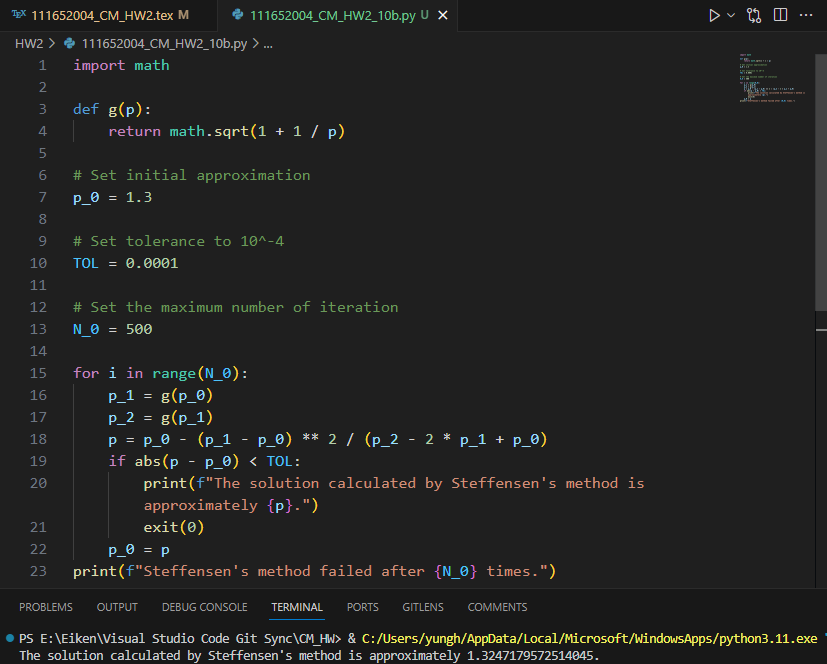
\includegraphics[width=0.9\textwidth]{problem_10b_py.png}
    \end{center}
    \qed
\end{enumerate}


\newpage
\begin{problem}\label{problem 11}
    Given a polynomial $P(x) = x^3-5x^2+8x-6$, do the following:
    \begin{enumerate}
        \item Evaluate $P(2)$, $P'(2)$, $P(4)$, and $P'(4)$ by Horner's method.
        \item Find the root of $P(x)$ with error less than $0.00001$ between $[2, 4]$ by using the Newton method with initial point $x_0 = 2$ and $x_0 = 4$. Determine which initial point may lead to the root.
        \item Deflate $P(x)$ into a quadartic polynomial by using the results in (b) and find the complex roots of $P(x)$.
        \item Perform one step of Müller's Method starting from initial $(0,P(0))$, $(1,P(1))$ and $(2,P(2))$.
        \item Implement a MATLAB\footnote{Prof. Wu says that we can use Python as well.} code of Müller's Method to find the complex root within error less than $0.00001$ and compare with the answer you find in (c).
    \end{enumerate}
\end{problem}
\textbf{Solution}.
\begin{enumerate}
    \item We first evaluate $P(2)$ and $P'(2)$. The table appears as follows:
    \begin{center}
        \begin{tabular}{|c|c|c|c|c|}
            \hline
            & Coefficient of $x^3$ & Coefficient of $x^2$ & Coefficient of $x$ & Constant term \\
            \hline
            $x_0=2$ & $a_3=1$ & $a_2=-5$ & $a_1=8$ & $a_0=-6$\\
            \hline
            &  & $b_3x_0=2$ & $b_2x_0=-6$ & $b_1x_0=4$\\
            \hline
            & $b_3=1$ & $b_2=-3$ & $b_1=2$ & $b_0=-2$\\
            \hline
        \end{tabular}
    \end{center}
    Hence $$P(x)=(x-2)(x^2-3x+2)-2.$$ We can therefore evaluate $P(2)=-2$ and $P'(2)=\left.x^2-3x+2\right|_{x=2}=0$. We now evaluate $P(4)$ and $P'(4)$. The table appears as follows:
    \begin{center}
        \begin{tabular}{|c|c|c|c|c|}
            \hline
            & Coefficient of $x^3$ & Coefficient of $x^2$ & Coefficient of $x$ & Constant term \\
            \hline
            $x_0=4$ & $a_3=1$ & $a_2=-5$ & $a_1=8$ & $a_0=-6$\\
            \hline
            &  & $b_3x_0=4$ & $b_2x_0=-4$ & $b_1x_0=16$\\
            \hline
            & $b_3=1$ & $b_2=-1$ & $b_1=4$ & $b_0=10$\\
            \hline
        \end{tabular}
    \end{center}
    Hence $$P(x)=(x-4)(x^2-x+4)+10.$$ We can therefore evaluate $P(4)=10$ and $P'(4)=\left.x^2-x+4\right|_{x=4}=16$.
    \item Since $P'(2)=0$, $x_0=2$ can't lead to the root. So we use $x_0=4$ only. By Python, the root is approximately $3.00002$.
    \begin{center}
        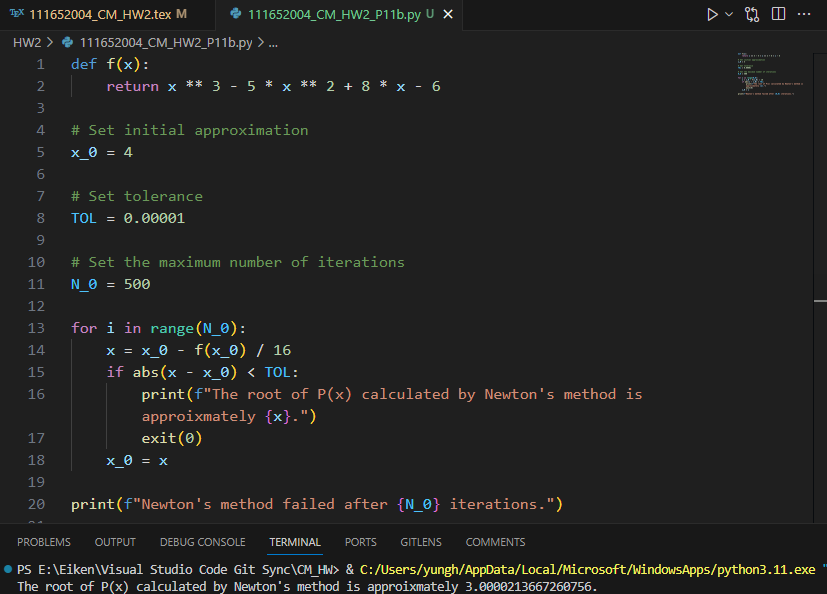
\includegraphics[width=0.9\textwidth]{problem_11b_py.png}
    \end{center}
    \item By the approximation, we first guess that $x=3$ is a solution to $P(x)=0$. Indeed, $P(3)=0$. Using the synthetic division, we have
    \begin{center}
        \begin{tabular}{|c|c|c|c|c|}
            \hline
            & Coefficient of $x^3$ & Coefficient of $x^2$ & Coefficient of $x$ & Constant term \\
            \hline
            $x_0=3$ & $a_3=1$ & $a_2=-5$ & $a_1=8$ & $a_0=-6$\\
            \hline
            &  & $b_3x_0=3$ & $b_2x_0=-6$ & $b_1x_0=6$\\
            \hline
            & $b_3=1$ & $b_2=-2$ & $b_1=2$ & $b_0=0$\\
            \hline
        \end{tabular}
    \end{center}
    which suggests that $P(x)=(x-3)(x^2-2x+2)$. By the quadratic formula, the complex solutions are $1\pm i$.
    \item We have $p_0=0$, $p_1=1$, and $p_2=2$. Set
    \begin{align*}
        h_1&=1-0=1,\\
        h_2&=2-1=1,\\
        \delta_1&=\dfrac{P(1)-P(0)}{1}=4,\\
        \delta_2&=\dfrac{P(2)-P(1)}{1}=0,\\
        d&=\dfrac{0-4}{1+1}=-2.
    \end{align*}
    Then
    \begin{align*}
        b&=0+1\cdot(-2)=-2,\\
        D&=\sqrt{(-2)^2-4\cdot P(2)\cdot(-2)}=2\sqrt{3}i.
    \end{align*}
    Since $|b-D|>|b+D|$, set $E=b-D=-2-2\sqrt{3}i$. Then $h=-2\cdot\dfrac{P(2)}{E}=\dfrac{2}{-1-\sqrt{3}i}=\dfrac{-1}{2}+\dfrac{\sqrt{3}}{2}i$. Thus $p=2+\dfrac{-1}{2}+\dfrac{\sqrt{3}}{2}i=\dfrac{3}{2}+\dfrac{\sqrt{3}}{2}i$.
    \item By Python, the root is approximately $1.000000+1.000000i$.
    \begin{center}
        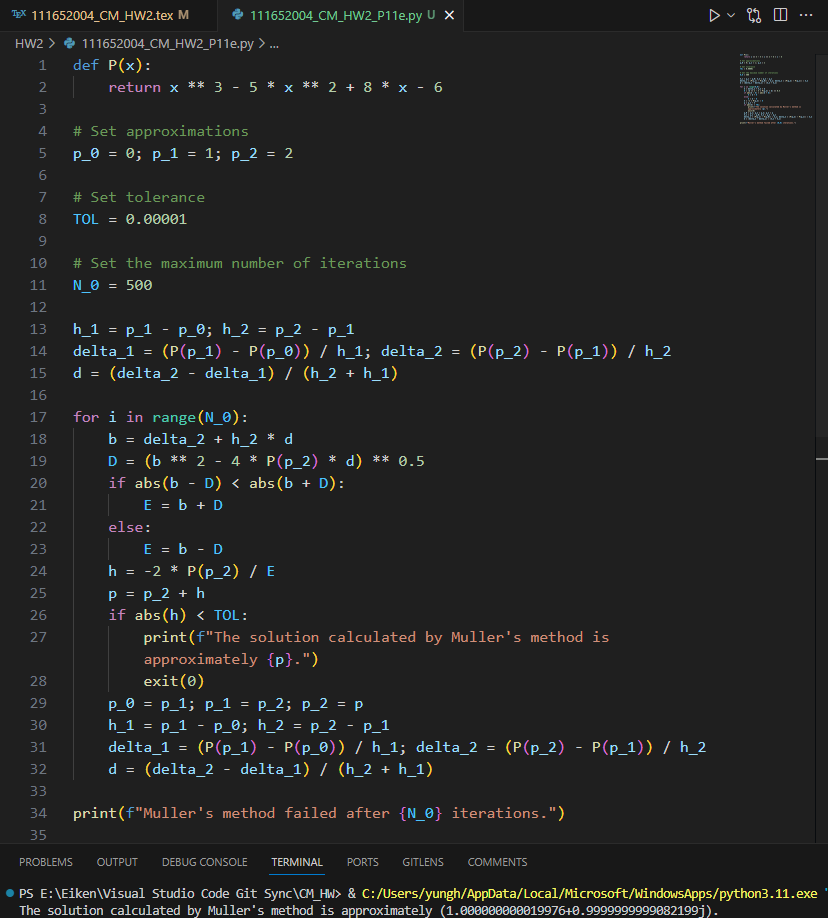
\includegraphics[width=0.9\textwidth]{problem_11e_py.png}
    \end{center}
    \qed
\end{enumerate}




\end{document}